%; whizzy paragraph -pdf xpdf -latex ./whizzypdfptex.sh
%; whizzy-paragraph "^\\\\begin{frame}\\|\\\\emtext"
% latex beamer presentation.
% platex, latex-beamer でコンパイルすることを想定。 

%     Tokyo Debian Meeting resources
%     Copyright (C) 2012 Junichi Uekawa
%     Copyright (C) 2011 Nobuhiro Iwamatsu

%     This program is free software; you can redistribute it and/or modify
%     it under the terms of the GNU General Public License as published by
%     the Free Software Foundation; either version 2 of the License, or
%     (at your option) any later version.

%     This program is distributed in the hope that it will be useful,
%     but WITHOUT ANY WARRANTY; without even the implied warreanty of
%     MERCHANTABILITY or FITNESS FOR A PARTICULAR PURPOSE.  See the
%     GNU General Public License for more details.

%     You should have received a copy of the GNU General Public License
%     along with this program; if not, write to the Free Software
%     Foundation, Inc., 51 Franklin St, Fifth Floor, Boston, MA  02110-1301 USA

\documentclass[cjk,dvipdfmx,12pt]{beamer}
\usetheme{Tokyo}
\usepackage{monthlypresentation}

\newenvironment{mycommandline}%
{\VerbatimEnvironment
  \begin{Sbox}\begin{minipage}{0.9\hsize}\begin{fontsize}{12}{12} \begin{BVerbatim}}%
{\end{BVerbatim}\end{fontsize}\end{minipage}\end{Sbox}
  \setlength{\fboxsep}{8pt}
% start on a new paragraph

\vspace{6pt}% skip before
\fcolorbox{dancerdarkblue}{dancerlightblue}{\TheSbox}

\vspace{6pt}% skip after
}
%end of commandline


%  preview (shell-command (concat "evince " (replace-regexp-in-string "tex$" "pdf"(buffer-file-name)) "&")) 
%  presentation (shell-command (concat "xpdf -fullscreen " (replace-regexp-in-string "tex$" "pdf"(buffer-file-name)) "&"))
%  presentation (shell-command (concat "evince " (replace-regexp-in-string "tex$" "pdf"(buffer-file-name)) "&"))

%http://www.naney.org/diki/dk/hyperref.html
%日本語EUC系環境の時
\AtBeginDvi{\special{pdf:tounicode EUC-UCS2}}
%シフトJIS系環境の時
%\AtBeginDvi{\special{pdf:tounicode 90ms-RKSJ-UCS2}}

\title{debug.debian.net}
\subtitle{大統一Debian勉強会}
\author{岩松 信洋\\iwamatsu@debian.org}
\date{2012年6月23日}
\logo{
\includegraphics[width=8cm]{image200607/openlogo-light.eps}}

\begin{document}

\frame{\titlepage{}}

\section{Agenda}
\begin{frame}{Agenda}
  \begin{itemize}
  \item 自己紹介
  \item Debianデバッグ情報用パッケージの現状
  \item Debianでのデバッグ情報パッケージについて
  \item 実装内容について
  \item 考えられる問題
  \item 今後の課題
  \item 質疑応答
\end{itemize}
\end{frame}

\section{自己紹介}
\emtext{自己紹介}

\begin{frame}{自己紹介}
  \begin{itemize}
  \item 岩松信洋 (twitter: @iwamatsu)
  \item Debian Project Official Developer
  \item Bluetooth, Mozc, OpenCV, libpng, Renesas/SH porter
  \item 大統一Debian勉強会実行委員長... なんだぜ?
  \end{itemize}
\end{frame}

\begin{frame}{こんなことありませんか?}
\begin{itemize}[<+->]
\item パッケージにバグがあったのでデバッグしてやろうと思ったらデバッグ情報がなかった
\item 「しょうがない、デバッグ情報を有効にしてやるか」と思い、再ビルドしたら再現しなかった
\item 古いパッケージだったので、ビルド用の環境構築がめんどう
\end{itemize}
\end{frame}

\begin{frame}
\begin{center}
\Huge{どうしたらいいのか、数秒考えてみた。}
\end{center}
\end{frame}

\begin{frame}[containsverbatim]

\begin{mycommandline}
      |
  \   __  /
  _  (m) _   ピコーン!
     |ミ|
  /  .`´  \
     ('A`)  もう全Debianパッケージで
     ノヽノヽ  デバッグ情報を提供して
       くく  しまえばいいんじゃね?

\end{mycommandline}
\end{frame}


\begin{frame}[containsverbatim]

\begin{center}
\Huge{とりあえず実装してみた、というのが今回の発表です。}
\end{center}
\end{frame}

\begin{frame}{デバッグ情報とは}
\begin{itemize}
\item 内部シンボル
\item 型の情報
\item ソースコードの行番号
\item etc
\end{itemize}
\end{frame}

\begin{frame}{デバッグ情報があると良い点}
\begin{itemize}
\item デバッガ(GDB)を使ったデバッグでより詳細なデバッグ情報を得ることができる
\item デバッグ情報を含めたバイナリを再度ビルドする必要がない
\item バイナリベースディストリビューションの場合、実際のバイナリとデバッグ情報が常に対になるので、バグの再現性が高くなる
\end{itemize}
\end{frame}

\begin{frame}{デバッグ情報があると悪い点}

\begin{itemize}
\item 実行ファイルにデバッグ情報が含まれるので実行ファイルのサイズが大きくなる
\item デバッグしない人にとっては不要なものが含まれることになる
\end{itemize}

\end{frame}

\begin{frame}{ようするにだな}
\begin{itemize}
\item すべての実行ファイルのデバッグ情報が提供されており
\item ユーザにとって必要のない情報がインストールされない仕組みがあれば
\item デバッグ情報パッケージはとても有益なものになるはず!!
\end{itemize}
\end{frame}

\emtext{Debianデバッグ情報用パッケージの現状}

\begin{frame}{Debian デバッグ情報用パッケージの現状}
\pause
\begin{itemize}
\item Debian ではいくつかのソースパッケージからデバッグ情報を含んだパッケージが提供されている
\item パッケージには\texttt{-dbg} というサフィックスが付いている
\item 特にデバッグ情報パッケージの提供に関するポリシーは決まっておらず、提供に関してはパッケージメンテナ次第
\end{itemize}
\end{frame}

\begin{frame}{Debian デバッグ情報用パッケージの現状}
2012/06/20 の時点での main
\begin{itemize}
\item バイナリパッケージ数 : 37520 個
\item ソースパッケージ数   : 18306 個
\item -dbg パッケージ数    : 1736 個
\item -dbg を提供しているソースパッケージ数 : 1401 個
\end{itemize}
\end{frame}

\begin{frame}{Debian デバッグ情報用パッケージの現状}
なぜ今まで提供されていなかったのか
\pause
\begin{itemize}
\item ディスク容量の問題
\item 回線の問題
\item そんなもん自分でビルドしろ、という風潮があった(ように思う)
\end{itemize}
これらはすでに過去の話。
\end{frame}

\begin{frame}{Debian デバッグ情報用パッケージの現状}
他のディストリビューションは?
\pause
\begin{itemize}
\item Fedoraでは \texttt{-debuginfo} というサフィックスを持ったパッケージが提供されている
\item Gentooではデフォルトでこれらの情報を生成し管理する仕組みがある
futures = splitdebug を指定
\end{itemize}
デバッグ情報の提供という点に関して他のディストリビューションに遅れを取っている。\\
\pause
これは問題。
\end{frame}

\section{Debianでのデバッグ情報パッケージについて}
\emtext{Debianでのデバッグ情報パッケージについて}

\begin{frame}{Debianでのデバッグ情報パッケージについて}
\begin{itemize}[<+->]
\item Debianではデバッグ情報パッケージは \texttt{-dbg} というサフィックスがついたパッケージ名を持つ
\item foo というアーキテクチャ依存のパッケージがあった場合、\texttt{foo} のデバッグ情報を持ったパッケージ名は\texttt{foo-dbg} になる
\item これらのパッケージに含まれるデータはどのように作成されるのか?
\end{itemize}
\end{frame}

\begin{frame}{Debianでのデバッグ情報パッケージについて}
デバッグ情報ファイル作成手順
\begin{center}
\includegraphics[width=1.0\hsize]{image2012-gum/ddebug-gum-image-data-debug-data00.eps}
\end{center}
\end{frame}

\begin{frame}{Debianでのデバッグ情報パッケージについて}
デバッグ情報ファイル作成手順
\begin{center}
\includegraphics[width=1.0\hsize]{image2012-gum/ddebug-gum-image-data-debug-data01.eps}
\end{center}
\end{frame}

\begin{frame}{Debianでのデバッグ情報パッケージについて}
デバッグ情報ファイル作成手順
\begin{center}
\includegraphics[width=1.0\hsize]{image2012-gum/ddebug-gum-image-data-debug-data02.eps}
\end{center}
\end{frame}

\begin{frame}{Debianでのデバッグ情報パッケージについて}
デバッグ情報ファイル作成手順
\begin{center}
\includegraphics[width=1.0\hsize]{image2012-gum/ddebug-gum-image-data-debug-data03.eps}
\end{center}
\end{frame}

\begin{frame}{Debianでのデバッグ情報パッケージについて}
デバッグ情報ファイル作成手順
\begin{center}
\includegraphics[width=1.0\hsize]{image2012-gum/ddebug-gum-image-data-debug-data04.eps}
\end{center}
\end{frame}

%\begin{itemize}
%\item Debian の \texttt{-dbg} パッケージで提供されているバイナリは動作するバイナリデータではなく、デバッグ情報のみを持ったデータ
%\item このファイルは \texttt{objdump --only-keep-debug}
%を実行することによって生成\\
%もちろん対象の実行ファイルはコンパイル時にデバッグ情報
%が付加されている必要がある。
%
%\item 次にデバッグ情報ファイルへのリンクを \texttt{strip} 済の実行可能形式に付加するために
%\texttt{objcopy --add-gnu-debuglink} を実行する。\\
%これによって、実行ファイルとデバッグ情報ファイルが対になる。
%
%\item GDB を使ってデバッグする際には実行ファイルとデバッグ情報ファイルはリンク
%しているので、デバッグ情報ファイルがインストールされているときは自動的に呼ばれ、デバッグ
%シンボルなどを読み込んでくれる。
%\end{itemize}
%\fi

\emtext{実装内容について}
%
%\begin{frame}{実装について}
%
%先に説明したようにに、すべての実行ファイルのデバッグ情報が提供されており
%ユーザにとって必要のない情報がインストールされない仕組みがあればよいので、
%これらに対応できる方法を考えました。以下で説明します。
%
%\end{frame}
%
\begin{frame}{全ての実行ファイルのデバッグ情報を提供するには?}
\pause
全てのパッケージで
\texttt{strip} された実行ファイルとデバッグ情報ファイルを持ったパッケージを構築すればよい
\end{frame}
\begin{frame}{Debianパッケージ構築順序}
\pause
\begin{itemize}[<+->]
\item パッケージ作成過程のどこかに手を加える必要がある
\item キーとなる処理の動作を簡単に説明
\begin{itemize}
\item dh\_strip
\item dh\_builddeb
\end{itemize}

\end{itemize}
\end{frame}

\begin{frame}{Debianパッケージ構築順序}
\begin{center}
 \\
\includegraphics[width=1.0\hsize]{image2012-gum/ddebug-gum-image-data-flow-only.eps}
\end{center}
\end{frame}

\begin{frame}{Debianパッケージ構築順序}
dh\_strip
\begin{center}
\includegraphics[width=1.0\hsize]{image2012-gum/ddebug-gum-image-data-dh-strip.eps}
\end{center}
\end{frame}

\begin{frame}{Debianパッケージ構築順序}
dh\_builddeb
\begin{center}
\includegraphics[width=1.0\hsize]{image2012-gum/ddebug-gum-image-data-dh-builddeb.eps} 
\end{center}
\end{frame}

%
%Debian の場合、パッケージはデバッグ情報が有効な状態(\texttt{gcc} だと\texttt{-g} オプション等)
%でビルドされます。そしてパッケージにされる時に \texttt{strip} (binutilsに含まれる)
%が \texttt{dh\_strip} から呼ばれ、実行ファイルやライブラリならデバッグ情報が削除され、
%パッケージ用のディレクトリにコピーされ、\texttt{dh\_builddeb} コマンドでパッケージ化されます。
%
%そして、配布される -dbg パッケージは \texttt{dh\_strip}を実行するときにデバッグ情報を提供する
%パッケージとして、\texttt{dh\_strip} のオプションとして指定されるか、debian/control ファイルに列挙されている
%パッケージ名のサフィックに \texttt{-dbg} が付いている場合、対象ファイルとして処理されます。
%

\begin{frame}{問題1}

%\item
自動生成したいデバッグ情報パッケージの情報をどのように生成するか
\pause
\begin{itemize}
\item Debianパッケージはdebian/control に記述されている情報を元に生成される
\item debian/contorl に生成されるパッケージ情報が書かれている必要がある
\end{itemize}
%\end{enumerate}
\end{frame}

\begin{frame}[containsverbatim]{対策: 自動生成したいデバッグ情報パッケージの情報をどのように生成するか}
\begin{itemize}
\item \texttt{dh\_strip} の処理の先頭で debian/control ファイルに
デバッグ情報パッケージファイルに関する情報を追記する処理を追加
\item デバッグ情報パッケージは対象のパッケージがアーキテクチャ依存(Architechture: all ではない)
である事とパッケージ名さえわかれば、パッケージ情報は自動生成できる
\end{itemize}
\end{frame}

\begin{frame}[containsverbatim]{対策: 自動生成したいデバッグ情報パッケージの情報をどのように生成するか}

\begin{commandline}
Package: hoge
Architecture: any
Depends: ${misc:Depends}
Description: hoge
\end{commandline}

\begin{commandline}
Package: hoge-dbg
Architecture: any
Section: debug
Priority: extra
Depends: hoge (= ${binary:Version}), ${misc:Depends}
Description: debugging symbols for hoge
 This package contains the debugging symbols for hoge
\end{commandline}

\end{frame}

\begin{frame}{問題2}
%\begin{enumerate}
%\item
\texttt{dh\_strip} でデバッグ情報パッケージが既に指定されている場合、
どのようにしてデバッグ情報用パッケージを自動生成するか
\pause
\begin{itemize}
\item dh\_stripは指定されているパッケージのみ、デバッグ情報ファイル作成処理を行う
\item 指定されていない場合は処理されない
\item 既にデバッグ情報用パッケージが提供されている場合でも、すべて提供されているわけではない。(ライブラリ用は提供されているが、ツール用は提供されていない場合がある)
\end{itemize}
%\end{enumerate}
\end{frame}

\begin{frame}{対策: \texttt{dh\_strip} でデバッグ情報パッケージ指定されている場合、自動生成したい -dbg パッケージ用のファイルをどのように生成するか}
\begin{itemize}[<+->]
\item アーキテクチャ依存のDebianパッケージは \bf{必ず} \texttt{dh\_strip} が呼ばれるため、ここで
処理をフックしてしまえば、デバッグ情報を提供するパッケージと用のデータと \texttt{strip} された
バイナリデータを分けることができる
\item 今回は \texttt{dh\_strip} の中身を改造し、全てのアーキテクチャ依存の
パッケージ用のデータを作成するように変更
\item \texttt{dh\_strip}でパッケージが指定されていても無視するように処理。なんでも処理をするように変更
\end{itemize}
\end{frame}

\begin{frame}{問題3}
%\begin{enumerate}
%\item 
自動生成したいデバッグ情報パッケージそのものをどのように生成するか
\pause
\begin{itemize}
\item dh\_strip で指定されているものしかデバッグパッケージ処理を行わない
\item dh\_strip 内でデバッグ情報が削除されてしまうため、削除される前にデバッグ情報を取得する必要がある
\end{itemize}

%\end{enumerate}
\end{frame}

\begin{frame}{対策: 自動生成したいデバッグ情報パッケージそのものをどのように生成するか}

\begin{itemize}
\item デバッグ情報パッケージの作成は \texttt{dh\_strip} 内で \texttt{dh\_builddeb} を呼び出すことで対応。
\item パッケージ名とパッケージ作成に必要なデータは揃っているため、
\texttt{dh\_builddeb -pデバッグ情報パッケージ名} を実行することで、パッケージが作成させる
\end{itemize}
\end{frame}

\begin{frame}{これってdebhelper 依存じゃないの?}
\pause
\begin{itemize}
\item これらの処理が行える前提条件として、debhelper に依存しているパッケージが対象になる
\item 現在ほとんどのパッケージが debhelper か CDBS に依存しており、CDBS は debhelper と
同時に使う事が多いため、問題はない。
\footnote{\url{http://people.debian.org/~cjwatson/dhstats.png}}
\end{itemize}
\end{frame}

\begin{frame}{パッケージサイズへの対応}
\pause
\begin{itemize}[<+->]
\item デバッグ情報は非常に大きい
\item \texttt{strip} されたバイナリの数倍以上のサイズになることもめずらしくない
\item どれぐらい大きいのか?
\item libjpeg8 で提供される libjpeg.so.8.4.0 のファイルの場合
\begin{itemize}
\item strip 前             : 約1.3MB 
\item strip 後             : 236KB\
\item デバッグ情報ファイル : 1.1MB 
\end{itemize}
\end{itemize}
\end{frame}
%------

\begin{frame}[containsverbatim]{パッケージサイズへの対応}
\begin{itemize}
\item パッケージサイズが大きく異なるので、パッケージを分けてもユーザが利用しているパッケージリポジトリ
と同じ場所・方法で提供してしまうと、ミラーに時間がかかるようになる
\item ユーザに不要なデータが格納されたリポジトリ情報を持たせることになる
\end{itemize}
\end{frame}

\begin{frame}[containsverbatim]{パッケージサイズへの対応}
\begin{itemize}
\item この問題を回避するためにリポジトリを分けることで対応
\item unstable で \texttt{strip} されているパッケージ(通常のパッケージ)は unstable とだけ指定し、
デバッグ情報を提供するパッケージは unstable/debug を指定する

\begin{commandline}
deb http://cdn.debian.or.jp/debian/ unstable main non-free
deb http://cdn.debian.or.jp/debian/ unstable/debug main
\end{commandline}

\item デバッグ情報が必要なユーザは unstable/debug を apt-line に追加することによってデバッグ情報用のパッケージが利用できるようになる
\end{itemize}
\end{frame}

\begin{frame}[containsverbatim]{パッケージサイズへの対応}
\begin{itemize}[<+->]
\item  パッケージが格納されるディレクトリのパスを変更することによって、
デバッグ情報のみを提供するミラーを構築することができ、debug 情報をミラーしないミラーサーバの負荷も今までと変わらない
\item すべてのミラーでデバッグ情報用パッケージをミラーする必要はない
\end{itemize}
\end{frame}

\begin{frame}{実装後について}

\begin{itemize}
\item これらを実装したシステムを reprepro + sbuild + rebuildd で構築した。
\item 現在stable/amd64のみをターゲットテストとして動作中。
\end{itemize}

\end{frame}

\emtext{考えられる問題}

\begin{frame}{セキュリティの問題}
\begin{itemize}[<+->]
\item ソースパッケージから作成されたバイナリバッケージの一覧は .changesファイルに
ファイルのハッシュと共に記述され、どのソースパッケージ(orig.tar.gz, dsc.diff.gz)
から作成されたのか分かるようになっている
\item 現時点での実装はバイナリパッケージ作成の課程で自動生成されるためのこれらの情報
とリンクしない
\item 仮にDebianで提供される場合、Buildd上でデバッグ情報ファイルパッケージが生成されるので個人的に
問題ないと思っているが、これらを紐付けるシステムがあるほうがより安全と言える
\end{itemize}

\end{frame}

\begin{frame}{バイナリの不一致}
\begin{itemize}[<+->]
\item 既存のシステムでは、\texttt{strip} されたバイナリと デバッグ情報が一致しない
ため、オフィシャルのバイナリと混ぜて使えないことが考えられる
\item 私が提供しているされているデバッグ情報パッケージを使う場合、
私が提供してる通常のパッケージも利用しないと意味がない
\item 今はこれをバージョンによる依存関係で回避
\item 最終的には buildd に入れてもらうことでデバッグ情報パッケージを自動生成することを
考えている
\end{itemize}

\end{frame}

\emtext{大きな落とし穴}

\begin{frame}
ヤッター!デキタヨー!思っていたら大きな落とし穴が待っていたのである...
\end{frame}

\begin{frame}
\Huge{そもそも debug.debian.netがあるんじゃね?}
\end{frame}

\begin{frame}{そもそも debug.debian.netがあるんじゃね?}
私のような凡人が考えるようなことは先人達はすでに考えているわけでして....\\
\pause
 \\
既に \url{http://debug.debian.net}というサービスがあり実装され、そして\color{red}{終了}していました。

\end{frame}

\begin{frame}{そもそも debug.debian.netがあるんじゃね?}
\begin{itemize}[<+->]
\item 実装と考えもほとんど同じ\\
	dh\_strip ですべてを処理するという考え
\item 大きく違うところはデバッグ情報パッケージの
サフィックスが\texttt{-dbg}ではなく、\texttt{-dbgsym}である
\item デバッグ情報を作成する部分が \texttt{dh\_builddeb} ではなく、\texttt{dpkg-deb} を使っている
\item \texttt{dh\_strip}を直接変更するのではなく、シンボリックリンクで
機能をオーバーライドさせている
\item ファイル拡張子が ddeb
\end{itemize}
\end{frame}

\begin{frame}{そもそも debug.debian.netがあるんじゃね?}
\begin{itemize}[<+->]
\item こちらの方がdebhelperに手を加えなくて済むのでこちらに乗り換え
\item 彼に連絡を取り、\url{debug.debian.net}再稼働させた
\item この発表が行われている頃には\sout{稼働しているはず}、まだしていなかった\\
  \url{http;//debug.debian.net} へデータコピーできてない\\
  \url{http://debug.nigauri.org} でビルド結果を参照可能
\end{itemize}
\end{frame}

\emtext{今後の課題}
\begin{frame}{今後の課題}

\begin{itemize}[<+->]
\item このままスタンドアロンでデバッグ情報パッケージを提供しても無駄なバイナリを生成するだけ
\item buildd にこのシステムを入れてもらい、dak で ディストリビューション/debug として
処理してもらうことが今後の大きな課題
\item このことについて来月開催される Debconf 12でBOF またはFTPチーム、wanna-builddチームと話をする予定
\item 誰か速いマシン貸してください
\end{itemize}
\end{frame}

\emtext{質疑応答}
\begin{frame}{質疑応答}

\begin{center}
なにか質問はありますか?
\end{center}

\begin{center}
ありがとうございました
\end{center}

\end{frame}

\end{document}
